% ==========================================================
\section{\textit{Models@run.time} via FMBP}
\label{sec:concept_fmbp}
% ==========================================================
 
A central goal of the proposed tool is to realize the \textit{models@run.time} paradigm~\cite{blair_models_2009, bencomo_modelsruntime_2019}.
In the context of behavioral programs combined with \gls{uvl} feature models, the graphical representation presented to the user through the \gls{glsp} editor must not only serve as a static configuration artifact.
Rather, it must continuously mirror the live state of the executing behavioral program.
Conversely, modifications the user applies to the graphical model should propagate to the running system.
 
FMBP provides the foundational layer for this integration~\cite{felber_comprehensible_2025}.
It is the only existing framework that combines the execution of behavioral programs with a \gls{uvl}-based configuration mechanism, making it the ideal candidate for realizing the \textit{models@run.time} approach in this graphical context.
The following section describes the conceptual design for extending FMBP to provide the runtime visibility and synchronization features required for an interactive model representation in the \gls{glsp} editor.

% ----------------------------------------------------------
\subsection{The Runtime State Visibility Problem}
\label{subsec:concept_fmbp_runtime_visibility}
% ----------------------------------------------------------
 
During execution, FMBP maintains all dynamic state internally.
In particular, two categories of runtime information are relevant for a live model representation.

\textbf{Dynamic environment attributes.}
As described in the previous sections, the \gls{uvl} feature model includes an \texttt{Env} feature whose variables capture measurements of the system's operational context.
While we initialize these values from the model at startup, the running FMBP framework continuously updates them in a local Python object~\cite{felber_tfelbrfmbp_2025}.
FMBP never modifies the underlying \gls{uvl} files during execution.
The current values exist exclusively in memory and are invisible to any external observer.

\textbf{Selected B-Events.}
The \gls{bp} paradigm centers on synchronizing b-threads through the declaration and selection of events.
Whenever the FMBP runtime selects a b-event for execution, this constitutes a meaningful behavioral transition.
Currently, in the examples provided by FMBP, such selections are only reported to the console as log output~\cite{felber_tfelbrfmbp_2025}.
The \gls{glsp} server has no means to observe these transitions and therefore cannot reflect them in the graphical model.

Both categories represent live runtime information that the \gls{glsp} server requires in order to uphold \textit{models@run.time}.
Since \gls{glsp} operates as a separate process and has no direct access to the FMBP Python runtime's object space, we must establish a communication mechanism.
That mechanism must proactively publish the runtime information.
By maintaining the \gls{glsp} server as an independent modeling component, the tool preserves its role as a general-purpose graphical editor.
This makes it extendable to multiple runtime systems without tight coupling to FMBP's internals.
This separation of runtime state from the graphical editor defines the synchronization problem that underpins RQ3.1 and RQ3.2.

% ----------------------------------------------------------
\subsection{Server-Sent Events as a publication mechanism}
\label{subsec:concept_fmbp_sse}
% ----------------------------------------------------------
 
A suitable solution for bridging the gap between the FMBP runtime and the \gls{glsp} server is \gls{sse}.
\gls{sse} is a lightweight, unidirectional HTTP-based streaming protocol in which a server pushes a stream of text-encoded events to any connected client~\cite{de_la_torre_using_2019}.
It is well supported, requires no custom protocol negotiation, and is straightforward to implement in Python~\cite{ramirez_sebastian_server-sent_nodate}.
Crucially, it aligns with the problem's directional nature.
The FMBP runtime is the sole authoritative source of truth for live state, and the \gls{glsp} server is a passive consumer that must apply updates as they arrive.
 
Under this approach, the FMBP runtime exposes an \gls{sse} endpoint.
The \gls{glsp} server subscribes to this endpoint at startup or when a user initiates a connection, receiving a continuous stream of events.
Upon receiving an event, the \gls{glsp} server applies the encoded state change to the internal model representation and triggers an update of the diagram.
This keeps the visual model synchronized with the executing program without requiring polling or file-based communication.
This publication mechanism provides the real-time update channel required to make RQ3.1 feasible in the graphical editor.

For the implementation, we use a single shared \gls{sse} port to enable concurrently running runtime models.
This constraint is necessary because one \gls{glsp} instance cannot reliably maintain separate connection settings for multiple model-specific \gls{sse} ports.
Therefore, each event carries the originating source file as metadata.
The source file then acts as the routing key that determines whether a received event belongs to the current \gls{glsp} instance.

% ----------------------------------------------------------
\subsection{Extending FMBP: Two Complementary Mechanisms}
\label{subsec:concept_fmbp_extensions}
% ----------------------------------------------------------
 
To realize the \gls{sse} publication, we introduce two architectural extensions to FMBP.
They are designed to be minimally invasive, preserving full backward compatibility with existing FMBP examples.
 
\paragraph{Decorator for Context Sources.}
We address the \texttt{Env} attribute problem by applying the \textit{decorator} design pattern~\cite{gamma_design_1993} to the existing context source abstraction in FMBP.
The framework uses a \texttt{ContextSource} that is injected into the \texttt{ContextConfigurationProvider} to supply environment data to the runtime~\cite{felber_comprehensible_2025}.
By wrapping the original context source in a decorated class, every invocation of the used \texttt{get\_data()} is intercepted~\cite{felber_tfelbrfmbp_2025}.
The decorator first delegates to the source to obtain the current context snapshot, and then publishes a corresponding \gls{sse} to the \gls{glsp} server before returning the data to the runtime.
The behavioral program itself requires no modification.
The decorator is inserted at the provider's construction site, making it trivially opt-in.
 
To avoid redundant network traffic, the decorator performs payload deduplication.
A new event is only emitted when the current snapshot differs from the previously published one.
This prevents the \gls{glsp} server from processing unnecessary updates when environment values are stable.
 
\paragraph{BPConfigurator Extension Mechanism.}
We address the b-event selection problem by a formal extension mechanism in the \texttt{BPConfigurator}, the central orchestration class and core component of FMBP~\cite{felber_comprehensible_2025}.
\texttt{BPConfigurator} subclasses \texttt{BProgramRunnerListener} from the \texttt{BPpy} package~\cite{yaacov_bppy_2023} and observes the program via two hooks. 
These are \texttt{starting(...)}, which is invoked once at program start, and \texttt{event\_selected(...)}, which is invoked for every selected b-event.
To integrate extensions, \texttt{BPConfigurator} is extended by passing a list of \texttt{BPConfiguratorExtension} objects at construction.
The extension protocol exposes the same hooks so extensions align with the configurator's lifecycle.
A concrete implementation of \texttt{BPConfiguratorExtension} should publish an SSE on each \texttt{event\_selected} call.
As with the decorator, extensions are registered at construction time and require no changes to core runtime logic.
Together, the decorator and configurator extensions provide the runtime hooks needed to observe both contextual updates and event selection, thereby directly advancing RQ3.1.

% ----------------------------------------------------------
\subsection{Interaction Flow}
\label{subsec:concept_fmbp_interaction_flow}
% ----------------------------------------------------------

\begin{figure}
	\centering
	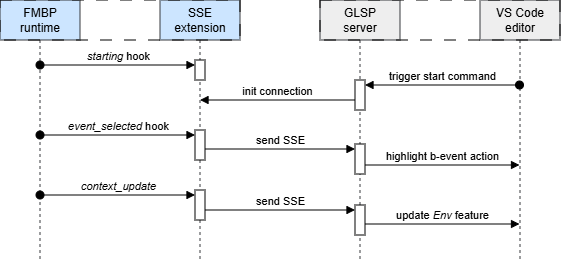
\includegraphics[width=0.9\textwidth]{figures/uml_fmbp_sequence_diagram.png}
	\caption{Sequence diagram showing the interaction between FMBP and GLSP.}
    \label{fig:bp-sequence-diagram}
\end{figure}

The combined interaction between FMBP, the \gls{sse} layer, and \gls{glsp} is illustrated in the sequence diagram in Figure~\ref{fig:bp-sequence-diagram}.
Upon program startup, \texttt{BPConfigurator} invokes the \texttt{starting} hook of all registered extensions, allowing the \gls{sse} server to initialize.
The \gls{glsp} server connects to the \gls{sse} endpoint and begins listening.
During execution, each selected a b-event triggers an \textit{event\_selected} server-sent event, which the \gls{glsp} server uses to highlight the corresponding element in the model.
Whenever the runtime samples a new context snapshot via the decorated context source, FMBP pushes a \textit{context\_update} event to the \gls{glsp} server, which updates the \texttt{Env} feature shown in the graphical model.
Both scenarios directly advance RQ3.1.

User edits in the graphical model are written back to the underlying \gls{uvl} files and are processed by the \gls{uvls} together with the \texttt{ConsistencyChecker}~\cite{felber_comprehensible_2025}.
The current FMBP implementation restricts certain updates.
Edits to the \texttt{Env} feature's measurement values are not applied to the live runtime~\cite{felber_tfelbrfmbp_2025}.
Although the changes do not affect the live system, a user may persist them to the \gls{uvl} file using \gls{glsp}'s save action.
To improve performance, we do not automatically persist context updates.
Variables explicitly designed for runtime reconfiguration are the attribute values of the \texttt{Config} feature.
Edits to these values are applied to the live runtime after persisting them in the \gls{uvl} file.
This write-back path defines the synchronization mechanism that answers RQ3.2.
This bidirectional coupling between the graphical model and the runtime state realizes the intended \textit{models@run.time} approach described in Section~\ref{sec:bg_models_at_runtime}.